\begin{frame}{}
    \begin{figure}
        \centering
        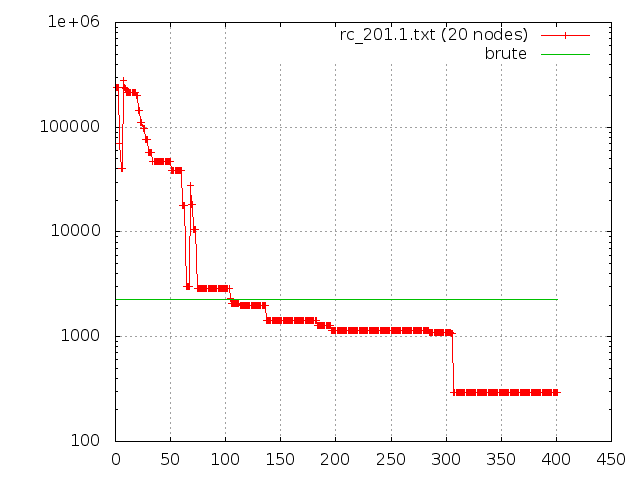
\includegraphics[width=8cm]{charts/rc_201_1.png}
        \caption{Wykres dla problemu rc\_201.1}
    \end{figure}
\end{frame}

\begin{frame}{}
    \begin{figure}
        \centering
        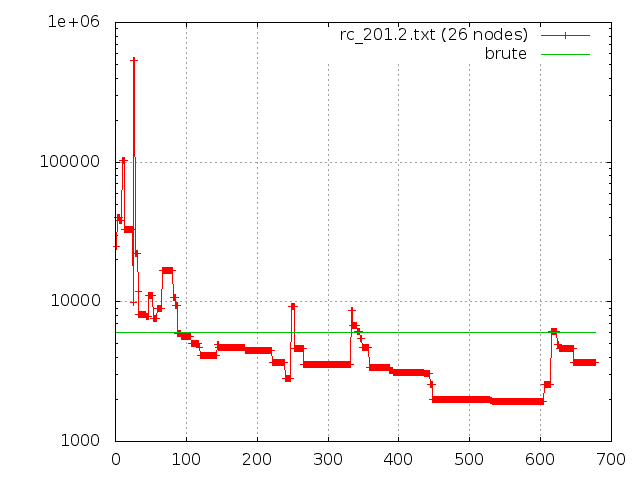
\includegraphics[width=8cm]{charts/rc_201_2.png}
        \caption{Wykres dla problemu rc\_201.2}
    \end{figure}
\end{frame}

\begin{frame}{}
    \begin{figure}
        \centering
        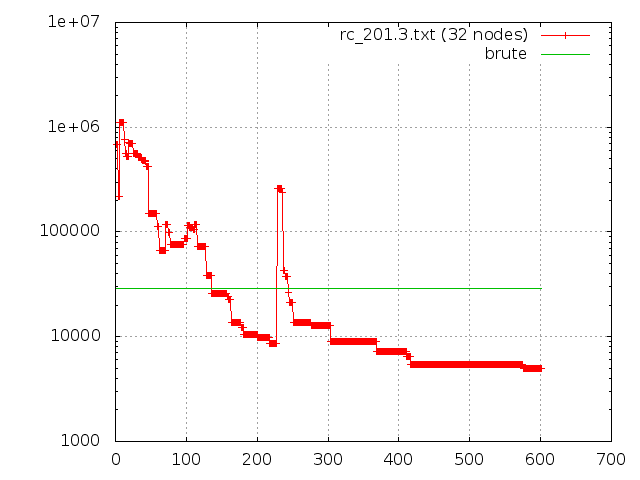
\includegraphics[width=8cm]{charts/rc_201_3.png}
        \caption{Wykres dla problemu rc\_201.3}
    \end{figure}
\end{frame}

\begin{frame}{}
    \begin{figure}
        \centering
        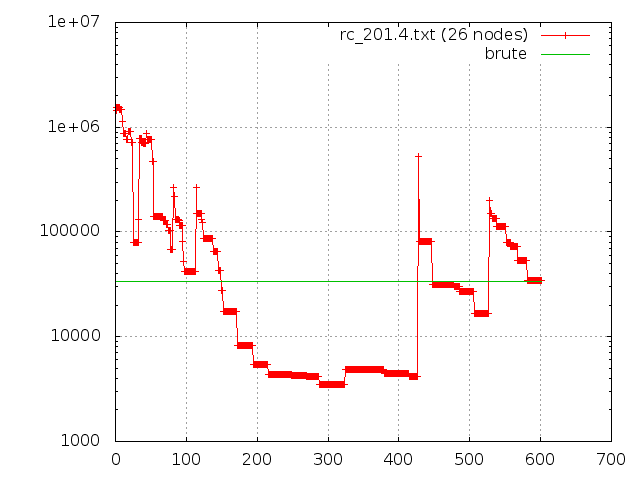
\includegraphics[width=8cm]{charts/rc_201_4.png}
        \caption{Wykres dla problemu rc\_201.4}
    \end{figure}
\end{frame}
